%
%  Erik Olsen
%
\documentclass[12pt,fullpage]{article}
\usepackage{fullpage}                                        % use all of the page for text 
\usepackage{psfrag}                                          % LaTeX graphics tool
\usepackage{pslatex}                                         % avoids the default cmr font
\usepackage{graphicx}                                        % graphics package 
\usepackage{epsfig}                                          % figures
\usepackage{epsfig} 
\usepackage{hyperref}
\usepackage{color}

\begin{document}

\noindent
{\bf Gamma--Poisson distribution} (from \color{blue}\url{http://www.math.wm.edu/~leemis/chart/UDR/UDR.html}\color{black})

\noindent
The shorthand $X \sim$ gamma--Poisson$(\alpha,\, \beta)$ is used to indicate that the
random variable~$X$ has the gamma--Poisson distribution with positive parameters $\alpha\  {\rm and}\  \beta$.
A gamma--Poisson random variable~$X$ has probability mass function 
$$
f(x) = \frac{\Gamma(x + \beta)\alpha ^ {\kern 0.08 em x}}{\Gamma(\beta)(1 + \alpha) ^ {\beta + x} x !} \qquad \qquad x = 0, 1, 2, \ldots
$$
for any $\alpha, \beta > 0$.
A gamma--Poisson random variable is a Poisson random variable with a random parameter $\mu$ which has the
gamma distribution with parameters $\alpha$ and $\beta$.
The probability mass function for three different parameter settings is illustrated below. \\

\begin{figure}[h!]
\begin{center}
\psfrag{labx}{$x$}
\psfrag{labf}{$f(x)$}
\psfrag{laba2}{$\alpha = 2$}
\psfrag{labb1}{$\beta = 1$}
\psfrag{laba1}{$\alpha = 1$}
\psfrag{labb2}{$\beta = 2$}
\psfrag{labb5}{$\beta = 5$}
\includegraphics[width=5.6in]{GammapoissonPlot.ps}
\end{center}
\end{figure}

\noindent
The cumulative distribution function on
the support of $X$ is
$$
F(x) = \sum_{w = 0} ^ x \frac{\Gamma (w + \beta)\alpha^ {w}}{\Gamma (\beta)(1 + \alpha)^{\beta + w} w !} \qquad \qquad x = 0, 1, 2, \ldots
$$
The moment generating function of X is
$$
M(t) = E[e^{\kern 0.08 em tx}] = (1 + \alpha - \alpha \kern 0.08 em e ^ {\kern 0.08 em t}) ^ {-\beta} \qquad \qquad -\infty < t < \infty. 
$$
The characteristic function of X is
$$
\phi(t) = E[e ^ {\kern 0.08 em i tx}] = (1 + \alpha - \alpha \kern 0.08 em  e ^ {\kern 0.08 em it}) ^ {-\beta} \qquad \qquad -\infty < t < \infty. 
$$
The population mean, variance, skewness, and kurtosis of $X$ are
$$
E[X] = \alpha \beta \qquad \qquad
V[X] = \alpha  \beta + \alpha ^ 2 \beta 
$$
$$
E\left[ \left( \frac{X - \mu} {\sigma} \right) ^ {\kern -0.08 em 3} \right] = \frac{1 + 2\alpha} {\sqrt{\alpha \beta (1 + \alpha)}} \qquad \qquad
E\left[ \left( \frac{X - \mu}{\sigma} \right) ^ {\kern -0.08 em 4} \right] = \frac{3 \alpha ^ 2 \beta + 6 \alpha ^ 2 + 3 \alpha \beta + 6 \alpha + 1}{\alpha \beta (1 + \alpha)}.
$$

%  There is no known source for the results from the moment generating function down

\vspace{0.1in}
%\noindent
%{\bf APPL verification:}
%The APPL statements
%\begin{verbatim}
%assume(beta > 0);
%assume(alpha > 0);
%X := [[GAMMA(x+beta)*alpha^x/(GAMMA(beta)*(1+alpha)^(x+beta)*factorial(x))], 
%	[0 .. infinity], ["Discrete", "PDF"]];
%CDF(X);
%MGF(X);
%Mean(X);
%Variance(X);
%Skewness(X);
%Kurtosis(X);
%\end{verbatim}
%verify the cumulative distribution function, moment generating function, population mean, variance, skewness, and kurtosis.
\end{document}
